\section{Methods}
\label{sec:Methods}

\subsection{Requirements \& FL Solution Comparison}
\label{subsec:MethodsRequirements}

% Deriving Requirements
Implementations of FL solutions in a real-world medical environment need to fulfill certain requirements. These are needed in order to utilize FL solutions in practical scenarios, meaning training a model across actual clinics. In this work, we derived these requirements by reviewing the related work, in particular synthetic and real-world implementations.

% own points - Some - Gesprochen mit Max, Klaus, Jonas
In addition, we add further requirements assessed from the experience of three domain experts in the field of FL and DL on medical image data. These requirements are considered by the experts to be relevant for the successful implementation of FL in a medical environment.

% Comparison
Based on the identified requirements, we compare multiple FL solutions, including our own proposed solution based on the JIP. Besides NVIDIA Clara Federated and PySyft, which have already been used in scientific publications (\Cref{sec:LitRev}), we also include the other FL solutions introduced in the related work. These solutions were already examined in earlier scientific publications of \cite{Li2019AProtection} and \cite{He2020FedML:Learning}, have a significant number of GitHub stars, and have an active repository with current contributions. Custom implementations are not considered further for comparison due to their lack of scalability. In order to gather the relevant information, we have intensively studied the provided documentation as well as tutorials and examples, if provided.



\subsection{PySyft Integration into the JIP}
\label{subsec:MethodsPySyftIntegration}
FL experiments can be conducted in various constellations. In order to realize our implementations, we had to make assumptions first.
% Explain general setting
We assume that there are participating clinics and a central instance, each of which hosts its own JIP installation. The communication always takes place via the central instance and not directly between the participants. This is, in particular, also the case with sequential computing plans.
% Data Scientist perspective
We assume that the data scientist who wants to conduct a federated experiment operates from the central instance.

% PySyft Components
The integration of PySyft is limited to its release version 0.2.9 because more recent versions do not yet support the local deployment of the computing instance.
This means that they can only be deployed via a public cloud service, which excludes the more recent PySyft versions from the usage in a secured medical clinic.
PySyft comes with three components.
\textit{PySyft-Notebook} is a jupyter-notebook environment with all required packages installed. It runs on the central instance and serves the data scientist as the development environment for his experiment.
\textit{PySyft-Grid} serves as the network to manage the communication. It can be accessed by the data scientist and searched for available data.
\textit{PySyft-Node} is the component that hosts the data, provides references to it in the \textit{PySyft-Grid} and performs the training computations. A node can be registered in a \textit{PySyft-Grid}, which then enables the data scientist to search and work with the provided references to the data hosted by the node.

The data can be marked with identification tags. All three components are provided by Openmined as ready-to-use container images and are easy to be integrated into the JIP without major adjustments due to the underlying Kubernetes cluster.To open the communication between the different nodes specific ports were excluded from the single sign-on.

% Kombination von beidem
For the experiments in this work, the \textit{PySyft-Node} was integrated into an Airflow DAG as an operator. Together with an operator to load the data into Airflow and another operator to provide the data, they form the DAG in the participating clinics. The data-providing operator performs the image transformations and then sends them all to the \textit{PySyft-Node}. After a given time, the operators stop, and the data is not provided in the \textit{PySyft-Grid} any further. The described process is illustrated as DAG in \Cref{fig:Dags} C.

% Training via Jupyter Notebook 
\textit{PySyft-Grid} and \textit{PySyft-Notebook} are hosted on the central instance.
From the notebook, it is then possible to search for the relevant data within \textit{PySyft-Grid} using the assigned identification tags. The received references to the data on the participating clinics can then be used as usual in PySyft to implement the training logic.

%\begin{figure}[h!]
\begin{figure}[htbp!]
%\begin{adjustbox}{width=1\textwidth}
    %\centerline{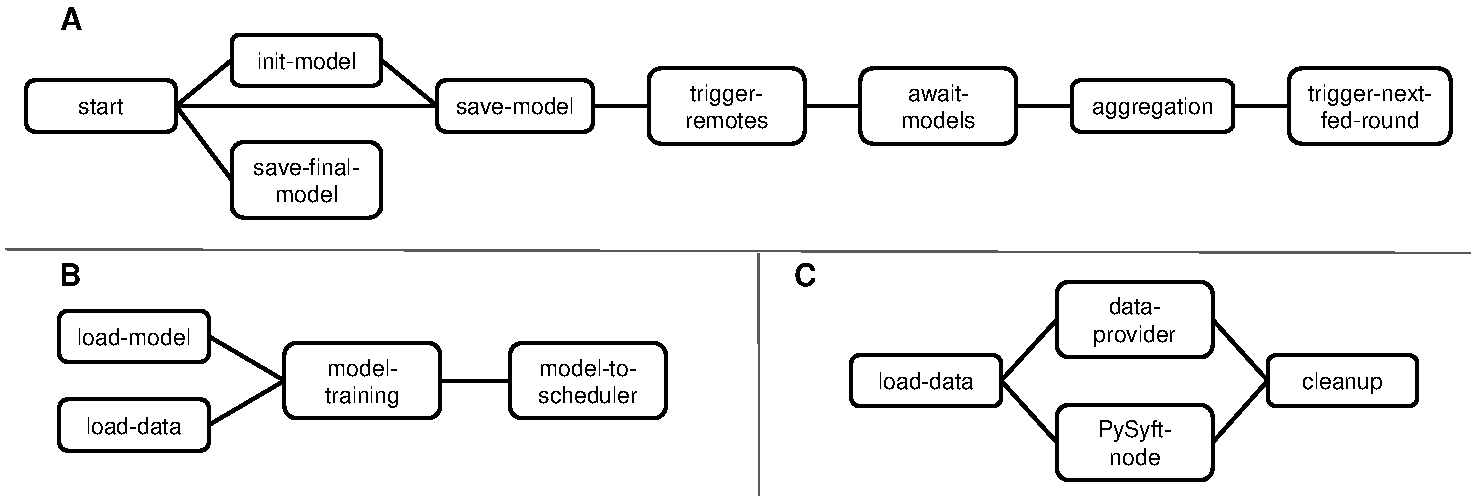
\includegraphics[width=1.95 \columnwidth]{1_Figures/dags.pdf}}
    \centerline{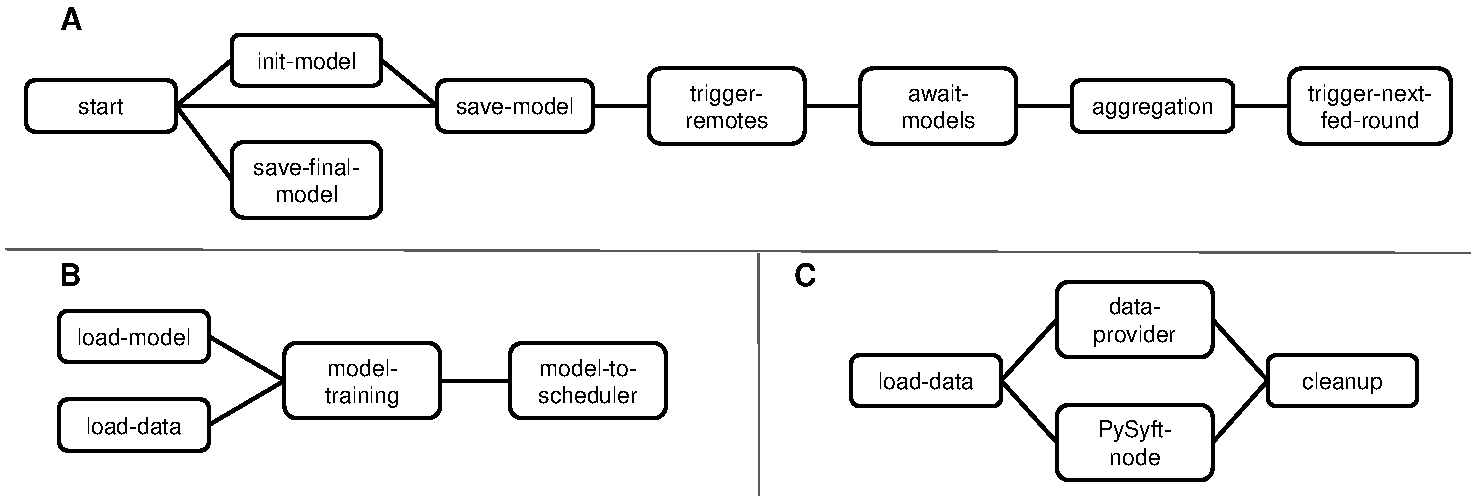
\includegraphics[width=1\textwidth]{1_Figures/dags.pdf}}
    \caption{Apache Airflow DAGs for JIP Federated (A \& B) and the JIP's PySyft integration (C). (A) DAG on central instance, which schedules the federated experiment and its individual process steps. (B) DAG on a participating institutions, which loads the local data and the consensus model from the central instance to execute the model training. When training is completed, the updated model is saved back to the central instance.  (C) DAG on a participating instance loading and providing its locally available data to the PySyft-Node, which then executes the computations during training. Note that the central instance of the PySyft integration hosts its PySyft-Notebook without being integrated into a DAG.}
%\end{adjustbox}
\label{fig:Dags}
\end{figure}



\subsection{JIP Federated}
\label{subsec:MethodsJIPFederated}

% shortly repeat setting
As with the PySyft integration, we assume a setting of multiple participating clinics and one central instance, all having their individual JIP installed. The data scientist implements and runs the experiment from the central instance.
% Ref to figure
The workflow on the central instance is illustrated in \Cref{fig:Dags} A, the training on the participants in \Cref{fig:Dags} B.

% Our JIP Federated implementation is 
We implemented JIP Federated in such way that it is primarily based on the two JIP components Apache Airflow and the object store MinIO as well as their corresponding APIs. Also here, some ports and URLs were whitelisted to enable a communication between the nodes. Different from the PySyft integration, the federated training is scheduled by an Airflow DAG on the central instance instead of a Jupyter-Notebook. An API call to Airflow is used to start the scheduler DAG and thus the federated experiment. With the API call, relevant parameters such as the number of federated rounds, corresponding epochs per round, and learning rate are provided.

% ### scheduler dag ####
The workflow on the central instance controls the processes of the experiment and can be described as follows (see \Cref{fig:Dags} A).
First, depending on the current round, either a new model is initialized  or the model of the previous round is directly stored into the object store.
In case it was the last round, the experiment is completed. Otherwise, it continues with the next operator.
% API Calls & Waiting
After saving the model, API calls are triggered on the participants' sites in order to start the corresponding training DAGs there. The relevant training information is also passed on to the participants. Subsequently, the workflow waits for the participants to send the models back to the central instance's object store. A regular check is made via the object store's its API to see whether all awaited models have already arrived.
% aggregation
When this is the case, the following operator performs the model aggregation and constructs the consensus model.
% completion
Before completing the current workflow, the DAG triggers itself for another run. Required data and information, such as the current federated round, are passed on to the next DAG. Thus, one federated round is represented by one run of the DAG on the central instance.

% training dag
At each participating clinic, identical training DAGs are implemented (see \Cref{fig:JIP} B).
The DAG starts with loading the data into Airflow. In parallel, a second operator accesses the object store of the central instance and loads the model from the previous round directly from there.
The operator to train the model brings the loaded data and model together and executes the training. After the local training is completed, the last operator saves the model back into the object store on the central instance.

% Usability
Due to the modularity of the DAGs, the individual operators can be reused for other experiments. In most cases, a developer only needs to customize the operators for aggregation and model training on the nodes to implement a new experiment.
%Apart from the operators for the experiments, all others are reusable in their current implemented form for further experiments. So a developer only needs to customize the operators for aggregation and training on the nodes to implement the new experiment.


\subsection{Development}
\label{subsec:Development}
Lorem ipsum dolor sit amet, consetetur sadipscing elitr, sed diam nonumy eirmod tempor invidunt ut labore et dolore magna aliquyam erat, sed diam voluptua. At vero eos et accusam et justo duo dolores et ea rebum. 


\subsection{Experiments, Algorithms \& Datasets}
\label{subsec:MethodsExperiments}

Two classification experiments were carried out to compare the JIP's PySyft integration and JIP Federated. These experiments aim to compare the runtime and thus the efficiency of the two solutions while achieving similar learning behavior and performance. Furthermore, a segmentation experiment on complex multi-modal medical images was conducted. 
We demonstrate that it is feasible to perform FL with the JIP on a standard benchmark dataset of medical images.
% General setting with three participants (in all experiments)
For all experiments, we assume that three participating institutes provide their local data. Further, in every federated round one epoch is trained on the available data.

% ### Runtime Experiments ###
The runtime experiments were conducted on two different publicly available datasets: the widely known Modified National Institute of Standards and Technology\footnote{\url{http://yann.lecun.com/exdb/mnist/}} (MNIST) dataset, consisting of 70,000 digit handwriting images (60,000 for training and 10,000 for testing), and the paediatric pneumonia dataset\footnote{\url{https://data.mendeley.com/datasets/rscbjbr9sj/3}} originally proposed by \cite{Kermany2018IdentifyingLearning}. It contains paediatric chest radiographs split into 5,232 samples for training and 624 for testing. The data is classified as either normal (with no signs of infection, 1,349 samples) or infected (bacterial or viral pneumonia, 3.883 samples). The test data contains 234 normal samples and 390 samples classified as infected. In order to use the datasets in a federated setting, non-overlapping subsets were formed. Each class in the training data was randomly divided into three parts and distributed among the participants. The test data was held out for final global testing after training. This process was applied on both datasets.
% dataset class distribution 
% total:    5,232 (3,883 pneumonia, 1,349 normal)
% training: ...
% testing:  624 (390 pneumonia, 234 normal)

% Applied transformations
For the training, image transformations were applied to both datasets. While the MNIST images were only normalised, the following transformations were performed on the pneumonia images.
Image resizing to $256 \times 256$ pixels,
random horizontal flipping,
random vertical flipping,
and image normalization.

For the MNIST experiments, the algorithm and training parameters were adopted from the basic MNIST example of PyTorch\footnote{\url{https://github.com/pytorch/examples/blob/master/mnist/main.py}; commit hash: 0f0c9131ca5c79d1332dce1f4c06fe942fbdc665}. Training was performed for 14 federated rounds using a batch size of 64 and a learning rate of $10^{-2}$. For the experiment on pneumonia radiographs, the ResNet18 (see \cite{He2016DeepRecognition}) architecture pre-trained on ImageNet was used, following \cite{Kaissis2021End-to-endImaging}. The model was trained for 40 federated rounds with a learning rate of $10^{-4}$ and a batch size of 8 (also used by the baseline for the processing time experiments in \cite{Kaissis2021End-to-endImaging}). Due to PySyft's limitation of not supporting momentum terms in the integrated release version, Stochastic Gradient Descent (SGD) was used as optimizer.
% Kaissis Baseline: "All times shown in white are relative to the baseline for a batch size of 8" - Haben sie als Baseline genutzt um den Zeitaufwand zu vergleichen

% For the classification experiments, two performance metrics are used. 
% TODO: Metric: Accuracy & AUR-ROC aufnehmen für die 

% ACCURACY
To measure the trained models performance on the test data, the metric \textit{Accuracy} was used. Its value represents the proportion of the correctly classified samples over all samples. The metric is defined as:
\begin{equation}
Accuracy=\frac{TP + TN}{TP + TN + FP + FN} \label{eq:accuracy}
\end{equation}
where TP = True Positive, FP = False Positive, TN = True Negative, FN = False Negative.
% AU-ROC
In addition, the receiver-operator-characteristic-area-under-the-curve (ROC-AUC) is measurend for the experiments on the slightly imbalanced pneunomia dataset.
The metric is a performance metric based on the receiver-operator-characteristic (ROC) curve, which represents possible combinations of true-positive-rate (TPR) and the false-postive-rate (FPR).
By mapping the FPR on the x-axis and the TPR on the y-axis, a curve is formed. The area underneath this curve is the ROC-AUC and its value ranges between 0 and 1 (higher is better). 


% Furthermore, the integrated PySyft version does not support graphical processing unit (GPU), thus, the experiments were carried on central processing unit (CPU) resources only.
Furthermore, all JIP instances for the experiments were set up identically, and training was carried out on the central processing unit (CPU). Computing resources of 10,000 Mi\footnote{\unexpanded{$1\ Mi\ (mebibyte) = 1024 \times 1024\ bytes$}} were allocated to each node, respectively training container, by the underlying Kubernetes.

% ### BraTS ###

In the federated segmentation experiment with JIP Federated, a U-Net (see \cite{Ronneberger2015U-net:Segmentation}) was trained to segment diagnosed gliomas in MRI scans of human brains. The U-Net architecture was set up with a channel sequence of ($16, 32, 64, 128, 256$) and convolution strides of size two. The number of residual units was set to two.
The results and training behavior is compared to an experiment where an identical U-Net architecture is trained on the centralized data using the same hyperparameter configuration.
In both cases, the models were trained for 500 epochs, respectively federated rounds.
% GPU
The model training computations were performed on graphical processing units (GPUs).
% Dataset description
The brain dataset from the \textit{Medical Segmentation Decathlon} was used. The dataset consists of a subset of the Brain Tumor Segmentation (BraTS \cite{Menze2015TheBRATS}) Challenge 2016 and 2017 data \citep{Antonelli2021TheDecathlon}. Besides unlabeled test samples, it contains 484 multi-modal MRI scans and their corresponding labels. 96 of the labeled samples were separated to serve as test data for measuring the model performance. For the experiment, three participating sites were established on individual server instances. Hence, the data was randomly sampled and divided into three non-overlapping subsets. Each instance was provided with 129 samples for training and 32 for testing. For centralized training, the identical data was merged into central datasets and then used for training and testing.
% bezeichnung der Daten <-- clear naming! 
In the remainder of this work, this data will be referred to as BraTS dataset.

% optimizer & reference to appendix for details
To train the model with this data, we used the Adam optimizer (see \cite{Kingma2014Adam:Optimization}) with a 
learninng rate of $10^{-4}$
and weight decay of $10^{-5}$.
% Applied transformations
For the model training, the brain scans undergo the following transformations.
Random vertical flipping,
random spacial cropping ($\textrm{with roi\_size} =  128 \times 128 \times 64$),
intensity normalization,
random intensity shifting,
random intensity scaling.
% ref to MONAI Tutorial
The parameters of the optimizer, the applied transformations, and the U-Net architecture were adopted from the 3D brain segmentation tutorial\footnote{\url{https://github.com/Project-MONAI/tutorials/blob/master/3d\_segmentation/brats\_segmentation\_3d.ipynb}; commit hash: d340613cea8b0f10b780694c636c1d7ff8f7658d}
%\footnote{https://github.com/Project-MONAI/tutorials}
of the Medical Open Network for AI (MONAI) Project\footnote{\url{https://monai.io/}}. After each federated round, the models are aggregated by applying \textit{Federated Averaging}.

% Optimizer state handling (keep local, agg, reset) --> Das hier ist neu!
When models are aggregated into a consensus model, the question of how to handle the used optimizer arises. For this \textit{optimizer state treatment}, three methods are apparent. As with the model, a consensus optimizer state could be derived from averaging the states of the participants. Alternatively, the optimizer state could be kept on the local instance only or reset for each new federated round. Based on the results shown in the work of \cite{Li2019Privacy-preservingSegmentation}, we decided to also reset the optimizer state before continuing a new federated round.
% sheller gibt nur die Werte für RESET und HOLD an - die sind sehr ähnlich, wie deutlich AGG besser ist wird nicht gesagt. Ich lasse Sheller weg, weil Li klar die Aussage trifft (und auch eben BraTS macht)
% \cite{Li2019Privacy-preservingSegmentation}: "For the treatment of momentum variables, restarting them at each federated round outperforms all the other variants" 

% Dice Score explaining!
As in all BraTS challenges, the \textit{Dice Coefficient} (DC) was used for the quantitative performance evaluation of the model.
This metric measures the overlap of two binary segmentation masks and ranges from 0 to 1 (higher is better). DC is defined as:
\begin{equation}
DC=\frac{2 |P \cap T|}{|P| + |T|} \label{eq:dice}
\end{equation}
where P is the prediction and T the ground truth mask. The DC is measured for all three (overlapping) tumor regions\footnote{In the medical segmentation decathlon, the label convention slightly differs from BraTS.}:
\begin{itemize}
    \item Enhancing tumor (ET): label 2
    \item Tumor core (TC): labels 2 and 3
    \item Whole tumor (WT): labels 1, 2 and 3
\end{itemize}

\begin{comment}
\begin{enumerate}
    \item Enhancing tumor (ET): label 2
    \item Tumor core (TC): labels 2 and 3
    \item Whole tumor (WT): labels 1, 2 and 3
\end{enumerate}
\end{comment}

% Table summerazis the chosesn parameter configurartions for all conducted experiments.
\Cref{tab:TrainingParameters} summarizes the chosen parameter configurations for all conducted experiments.
Note that apart from the listed parameters, the Adam optimizer was used with its PyTorch default values for the segmentation experiment.

\begin{table}[htbp]
\begin{adjustbox}{width=1.0\textwidth}
  \centering
  \begin{tabular}{ccccccc}
  Experiment & Federated Rounds & Epochs per Round & Optimizer & Batch Size & Learning Rate & Weight Decay \\
  \hline \\[-2.5ex] %[-1.5ex]
  MNIST     & 14    & 1 & SGD   & 64 & $10^{-2}$ & - \\
  Pneunomia & 40    & 1 & SGD   & 8  & $10^{-4}$ & - \\
  BraTS     & 500   & 1 & Adam  & 2  & $10^{-4}$ & $10^{-5}$ \\
 \end{tabular}
 \end{adjustbox}
 \caption{Training parameters for conducted experiments on MNIST, pneumonia and BraTS data.}
 \label{tab:TrainingParameters}
\end{table}
